\documentclass[11pt]{article}

\usepackage[margin=1.6cm]{geometry}
\usepackage{amsmath,amssymb,amsthm}
\usepackage[hidelinks]{hyperref}
\usepackage[most]{tcolorbox}
\usepackage[]{cancel}
\usepackage{tikz-feynman}
\usepackage{slashed}
\tikzfeynmanset{compat=1.1.0}
\newenvironment{solution}[1][]{\begin{proof}[\textbf{Solution}]}{\end{proof}}
% --- Rounded box style for each problem (whole statement) ---
\tcbset{
    problem/.style={
        enhanced,
        boxrule=0.7pt,
        arc=3mm,
        left=3mm,right=3mm,top=2mm,bottom=2mm,
        colback=white,
        colframe=black,
        before skip=10pt,
        after skip=6pt,
    }
}



\begin{document}
\begin{center}
    {\LARGE \textbf{Solution Manual of Problem Set 14} \par}
    \vspace{1em}
    {\large Bufan Zheng\\ \href{mailto:bufan@g.ecc.u-tokyo.ac.jp}{\texttt{bufan@g.ecc.u-tokyo.ac.jp}} \par}
\end{center}



\begin{tcolorbox}[problem]
\textbf{1.} Draw the two tree-level QED diagrams contributing to Compton scattering $e^-\gamma\to e^-\gamma$, label momenta, and write down the amplitude as a sum of two terms.
\end{tcolorbox}
\begin{solution}[14.1]
	We have the following Feynman diagrams:
	
\begin{figure}[h]
	\centering
	
	% s-channel
	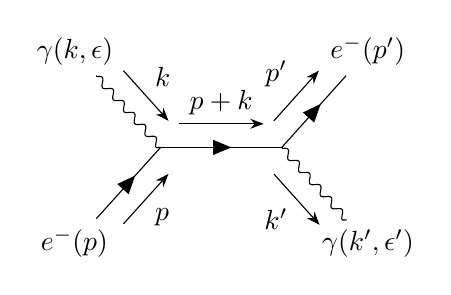
\begin{tikzpicture}[baseline=(current bounding box.center)]
		\begin{feynman}
			\diagram [horizontal=a to b] {
				i1 [particle=$e^-(p)$] -- [fermion, momentum'=$p$] a
				-- [fermion, momentum=$p+k$] b
				-- [fermion, momentum=$p'$] f1 [particle=$e^-(p')$],
				i2 [particle={$\gamma(k,\epsilon)$}] -- [photon, momentum=$k$] a,
				b -- [photon, momentum'=$k'$] f2 [particle={$\gamma(k',\epsilon')$}],
			};
		\end{feynman}
	\end{tikzpicture}
	\hspace{1.2cm}
	% u-channel
	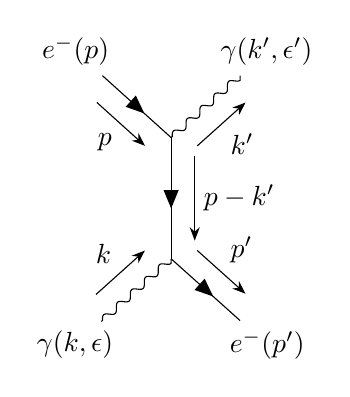
\begin{tikzpicture}[baseline=(current bounding box.center)]
		\begin{feynman}
			\diagram [vertical=a to b] {
				i1 [particle=$e^-(p)$] -- [fermion, momentum'=$p$] a,
				a -- [fermion, momentum=$p-k'$] b,
				b -- [fermion, momentum=$p'$] f1 [particle=$e^-(p')$],
				a -- [photon, momentum'=$k'$] f2 [particle={$\gamma(k',\epsilon')$}],
				i2 [particle={$\gamma(k,\epsilon)$}] -- [photon, momentum=$k$] b,
			};
		\end{feynman}
	\end{tikzpicture}
	
\end{figure}

	By Feynman rules, \textbf{MY FINAL ANSWER IS}:
		\[
		\boxed{
		\begin{gathered}
		i\mathcal M_s
		=(-ie)^2\,\bar u(p')\,
		\slashed\epsilon^{\,*}(k')\,
		\frac{i(\slashed p+\slashed k+m)}{(p+k)^2-m^2+i\varepsilon}\,
		\slashed\epsilon(k)\,
		u(p),\\
		i\mathcal M_u
		=(-ie)^2\,\bar u(p')\,
		\slashed\epsilon(k)\,
		\frac{i(\slashed p-\slashed k'+m)}{(p-k')^2-m^2+i\varepsilon}\,
		\slashed\epsilon^{\,*}(k')\,
		u(p).\\
	i\mathcal M = i\mathcal M_s + i\mathcal M_u,
			\end{gathered}}
	\]
\end{solution}



\begin{tcolorbox}[problem]
\textbf{2.} Using on-shell conditions, show that the tree amplitude is gauge invariant, replacing $\epsilon^\mu(k)\to k^\mu$ gives zero (Ward identity at tree level).
\end{tcolorbox}
\begin{solution}[14.2]
	We need to prove that $i\mathcal{M}({\epsilon\to k}=0)$. Since the external particles are on-shell, so we can use the following Dirac equations:
	
	% (1) External Dirac equations (on-shell spinors)
	\[
	(\slashed p-m)\,u(p)=0,
	\qquad
	\bar u(p')\,(\slashed p'-m)=0.
	\]
	\textbf{MY FINAL ANSWER IS}:
	% 1) 把入射光子的极化替换为动量, \slashed\epsilon(k)\to\slashed k
	\begin{align*}
		i\mathcal M\Big|_{\slashed\epsilon(k)\to\slashed k}
		&=(-ie)^2\,\bar u(p')\Bigg[
		\slashed\epsilon^{\,*}(k')\,
		\frac{i(\slashed p+\slashed k+m)}{(p+k)^2-m^2+i\varepsilon}\,
		\slashed k
		+\slashed k\,
		\frac{i(\slashed p-\slashed k'+m)}{(p-k')^2-m^2+i\varepsilon}\,
		\slashed\epsilon^{\,*}(k')
		\Bigg]u(p)
		\\
		&=(-ie)^2\,\bar u(p')\Bigg[
		\slashed\epsilon^{\,*}(k')\,
		\frac{i(\slashed p+\slashed k+m)}{(p+k)^2-m^2+i\varepsilon}\,
		\Big((\slashed p+\slashed k-m)-(\slashed p-m)\Big)
		\\
		&\qquad\qquad
		+\Big((\slashed p'-m)-(\slashed p-\slashed k'-m)\Big)\,
		\frac{i(\slashed p-\slashed k'+m)}{(p-k')^2-m^2+i\varepsilon}\,
		\slashed\epsilon^{\,*}(k')
		\Bigg]u(p)
		\\
		&=(-ie)^2\,\bar u(p')\Bigg[
		\slashed\epsilon^{\,*}(k')\,
		\frac{i(\slashed p+\slashed k+m)(\slashed p+\slashed k-m)}{(p+k)^2-m^2+i\varepsilon}
		-(\slashed p-\slashed k'-m)\,
		\frac{i(\slashed p-\slashed k'+m)}{(p-k')^2-m^2+i\varepsilon}\,
		\slashed\epsilon^{\,*}(k')
		\Bigg]u(p)
		\\
		&=(-ie)^2\,\bar u(p')\Bigg[
		\slashed\epsilon^{\,*}(k')\,
		\frac{i\big((p+k)^2-m^2\big)}{(p+k)^2-m^2+i\varepsilon}
		-\frac{i\big((p-k')^2-m^2\big)}{(p-k')^2-m^2+i\varepsilon}\,
		\slashed\epsilon^{\,*}(k')
		\Bigg]u(p)
		\\
		&=(-ie)^2\,i\,\bar u(p')\slashed\epsilon^{\,*}(k')u(p)
		-(-ie)^2\,i\,\bar u(p')\slashed\epsilon^{\,*}(k')u(p)
		\\
		&=0.
	\end{align*}
	% 2) 把出射光子的极化替换为动量, \slashed\epsilon^{\,*}(k')\to\slashed k'
	
	\begin{align*}
		i\mathcal M\Big|_{\slashed\epsilon^{\,*}(k')\to\slashed k'}
		&=(-ie)^2\,\bar u(p')\Bigg[
		\slashed k'\,
		\frac{i(\slashed p+\slashed k+m)}{(p+k)^2-m^2+i\varepsilon}\,
		\slashed\epsilon(k)
		+\slashed\epsilon(k)\,
		\frac{i(\slashed p-\slashed k'+m)}{(p-k')^2-m^2+i\varepsilon}\,
		\slashed k'
		\Bigg]u(p)
		\\
		&=(-ie)^2\,\bar u(p')\Bigg[
		\Big((\slashed p+\slashed k-m)-(\slashed p'-m)\Big)\,
		\frac{i(\slashed p+\slashed k+m)}{(p+k)^2-m^2+i\varepsilon}\,
		\slashed\epsilon(k)
		\\
		&\qquad\qquad
		+\slashed\epsilon(k)\,
		\frac{i(\slashed p-\slashed k'+m)}{(p-k')^2-m^2+i\varepsilon}\,
		\Big((\slashed p-m)-(\slashed p-\slashed k'-m)\Big)
		\Bigg]u(p)
		\\
		&=(-ie)^2\,\bar u(p')\Bigg[
		\frac{i(\slashed p+\slashed k-m)(\slashed p+\slashed k+m)}{(p+k)^2-m^2+i\varepsilon}\,
		\slashed\epsilon(k)
		-\slashed\epsilon(k)\,
		\frac{i(\slashed p-\slashed k'+m)(\slashed p-\slashed k'-m)}{(p-k')^2-m^2+i\varepsilon}
		\Bigg]u(p)
		\\
		&=(-ie)^2\,\bar u(p')\Bigg[
		\frac{i\big((p+k)^2-m^2\big)}{(p+k)^2-m^2+i\varepsilon}\,
		\slashed\epsilon(k)
		-\slashed\epsilon(k)\,
		\frac{i\big((p-k')^2-m^2\big)}{(p-k')^2-m^2+i\varepsilon}
		\Bigg]u(p)
		\\
		&=(-ie)^2\,i\,\bar u(p')\slashed\epsilon(k)u(p)
		-(-ie)^2\,i\,\bar u(p')\slashed\epsilon(k)u(p)
		\\
		&=0.
	\end{align*}
\end{solution}

\begin{tcolorbox}[problem]
\textbf{3.} In covariant $\xi$ gauge, show explicitly that the amplitude is independent of $\xi$ (at tree level) because external photons appear only through polarization vectors.
\end{tcolorbox}
\begin{solution}[14.3]
	In covariant $\xi$ gauge the gauge-fixing term is
	\[
	\mathcal L_{\text{gf}}=-\frac{1}{2\xi}\,(\partial_\mu A^\mu)^2,
	\]
	which modifies only the photon propagator,
	\[
	D_{\mu\nu}(q)=\frac{-i}{q^2+i\varepsilon}\left(\eta_{\mu\nu}-(1-\xi)\frac{q_\mu q_\nu}{q^2+i\varepsilon}\right).
	\]
	Hence any $\xi$-dependence of an amplitude can only come from internal photon lines.
	
	For tree-level Compton scattering $e^-\gamma\to e^-\gamma$, the two diagrams contain
	only the QED vertices $(-ie\gamma^\mu)$ and internal \emph{electron} propagators
	\[
	S_F(q)=\frac{i(\slashed q+m)}{q^2-m^2+i\varepsilon},
	\]
	which is $\xi$--independent. While the photons are \emph{external} and enter only through polarization vectors
	$\epsilon^\mu(k)$ and $\epsilon^{*\nu}(k')$. So we only need to care about the following sub-diagram:
	\[
	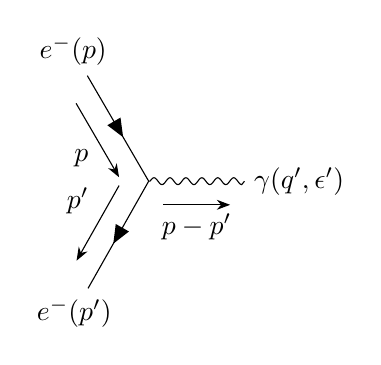
\begin{tikzpicture}[baseline=(current bounding box.center)]
		\begin{feynman}
			\diagram [horizontal=a to f] {
				i1 [particle=$e^-(p)$] -- [fermion, momentum'=$p$] a
				-- [fermion, momentum'=$p'$] i2 [particle=$e^-(p')$],
				a -- [photon, momentum'=$p-p'$] f [particle={$\gamma(q',\epsilon')$}],
			};
		\end{feynman}
	\end{tikzpicture}
	\quad\supset\quad q_\mu \bar u(p')\gamma^\mu u(p)
	\]
	
	\[
	\begin{aligned}
		q_\mu \bar u(p')\gamma^\mu u(p)
		&=\bar u(p')\,\slashed q\,u(p)\\
		&=\bar u(p')(\slashed p'-\slashed p)u(p)\\
		&=\bar u(p')\big[(\slashed p'-m)-(\slashed p-m)\big]u(p)\\
		&=\bar u(p')(\slashed p'-m)u(p)-\bar u(p')(\slashed p-m)u(p)\\
		&=0.
	\end{aligned}
	\]
	Therefore, any term in $D_{\mu\nu}$ that is proportional to the momentum $k_\mu$ does not contribute to the amplitude. Since the $\xi$--dependent part of $D_{\mu\nu}$ is precisely of this form, the final amplitude is $\xi$--independent.
\end{solution}

\begin{tcolorbox}[problem]
\textbf{4.} In $D$ dimensions, show that a physical photon has $D-2$ polarizations. Give a simple argument in momentum space.
\end{tcolorbox}
\begin{solution}[14.4]
	The polarization vector of a photon is constrained by the following on-shell equation:
	\[
	k^\mu \epsilon_\mu = 0,
	\]
	which reduces the degrees of freedom to $D-1$. Due to gauge invariance:
	\[
	\epsilon^\mu \sim \epsilon^\mu + k^\mu,
	\]
	the physical degrees of freedom of the photon are eventually reduced to $D-2$.
\end{solution}
\begin{tcolorbox}[problem]
\textbf{5.} Write the polarization sum for external photons in a way consistent with gauge invariance (i.e.\ explain why you can effectively use $-\eta^{\mu\nu}$ inside gauge-invariant expressions).
\end{tcolorbox}
\begin{solution}[14.5]
consider an arbitrary QED process involving an external photon with momentum $k$:
\[
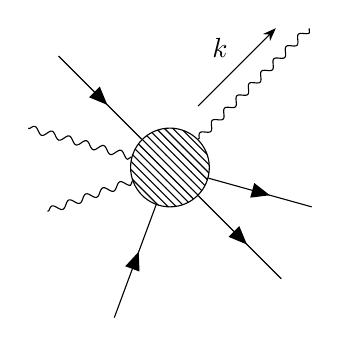
\begin{tikzpicture}[baseline=(current bounding box.center)]
	\begin{feynman}
		% 1. 定义中心标准 blob
		% 可以通过 minimum size 稍微调整它的大小
		\vertex [blob, minimum size=1cm] (c) {};
		
		% 2. 定义周围的顶点位置（手动指定以模拟原图的随意感）
		% 左侧入射
		\vertex [above left=2cm of c] (i1);
		\vertex [left=1.8cm of c, yshift=0.5cm] (i2);
		\vertex [below left=2.2cm of c, yshift=1cm] (i3);
		\vertex [below left=1cm of c,yshift=-1.2cm, rotate=-20] (i4);
		
		% 右侧出射
		% 关键的带动量 k 的光子顶点位置
		\vertex [above right=2.5cm of c] (o_k); 
		% 其他出射粒子
		\vertex [below right=2cm of c] (o2);
		\vertex [right=1.8cm of c, yshift=-0.5cm] (o3);
		
		% 3. 绘制连接线 (使用 \diagram* 手动模式)
		\diagram* {
			% 入射粒子 (混合直线和波浪线)
			(i1) -- [fermion] (c),
			(i2) -- [photon] (c),
			(i3) -- [photon] (c),
			(i4) -- [fermion] (c),
			
			% 关键：带有动量 k 的出射光子
			% momentum 选项会自动添加箭头和标签
			(c) -- [photon, momentum=\(k\)] (o_k),
			
			% 其他出射粒子
			(c) -- [fermion] (o2),
			(c) -- [fermion] (o3),
		};
	\end{feynman}
\end{tikzpicture}
	\qquad= i\mathcal{M}(k)\equiv i\mathcal{M}^\mu(k)\epsilon_\mu^*(k)
\]
We can choose the reference frame such that $k^\mu=(k,0,0,k)$. Hence the polarization vector is:
\[
\epsilon_1^\mu=(0,1,0,0);\quad\epsilon_2^\mu=(0,0,1,0).
\]
With these conventions, we have
\[
\begin{aligned}
	\sum_\epsilon\lvert\epsilon_\mu^*(k)\mathcal{M}^\mu(k)\rvert^2&=\sum_{\epsilon}\epsilon_{\mu}^{*}\epsilon_{\nu}\mathcal{M}^{\mu}(k)\mathcal{M}^{\nu*}(k)\\&=|\mathcal{M}^{1}|^{2}+|\mathcal{M}^{2}|^{2}\\&=|\mathcal{M}^1|^2+|\mathcal{M}^2|^2+|\mathcal{M}^3|^2-|\mathcal{M}^0|^2\\&=-g_{\mu\nu}\mathcal{M}^{\mu}(k)\mathcal{M}^{\nu*}(k).
\end{aligned}
\]
Here, we used the Ward identity:
$$
k^\mu \mathcal{M}_\mu=k\mathcal{M}^0(k)-k\mathcal{M}^3(k)=0\Rightarrow \mathcal{M}^0=\mathcal{M}^3
$$
\textbf{MY FINAL ANSWER IS}:
\[
\boxed{
	\sum_\text{polarizations}\epsilon_\mu^*\epsilon_\nu\:\longrightarrow\:-\eta_{\mu\nu}
}
\]
\end{solution}
\begin{tcolorbox}[problem]
\textbf{6.} Compute $|{\cal M}|^2$ averaged over initial electron spin and initial photon polarizations and summed over finals, keeping $D$ symbolic up to the point where $D-2$ appears.
\end{tcolorbox}
\begin{solution}[14.6]
	\[
\begin{aligned}
	i\mathcal{M} &= \bar{u}(p')(-ie\gamma^\mu)\epsilon^*_\mu(k') \frac{i(\slashed{p} + \slashed{k} + m)}{(p+k)^2 - m^2} (-ie\gamma^\nu)\epsilon_\nu(k)u(p) \\
	&\quad + \bar{u}(p')(-ie\gamma^\nu)\epsilon_\nu(k) \frac{i(\slashed{p} - \slashed{k}' + m)}{(p-k')^2 - m^2} (-ie\gamma^\mu)\epsilon^*_\mu(k')u(p) \\[10pt]
	&= -ie^2 \epsilon^*_\mu(k') \epsilon_\nu(k) \bar{u}(p') \left[ \frac{\gamma^\mu (\slashed{p} + \slashed{k} + m) \gamma^\nu}{(p+k)^2 - m^2} + \frac{\gamma^\nu (\slashed{p} - \slashed{k}' + m) \gamma^\mu}{(p-k')^2 - m^2} \right] u(p).
\end{aligned}
\]
 Since $p^2 = m^2$ and $k^2 = 0$, the denominators of the propagators are
\[
(p+k)^2 - m^2 = 2p \cdot k \quad \text{and} \quad (p-k')^2 - m^2 = -2p \cdot k'.
\]
To simplify the numerators, we use a bit of Dirac algebra:
\begin{align*}
	(\slashed{p} + m)\gamma^\nu u(p) &= (2p^\nu - \gamma^\nu \slashed{p} + \gamma^\nu m)u(p) \\
	&= 2p^\nu u(p) - \gamma^\nu (\slashed{p} - m)u(p) \\
	&= 2p^\nu u(p).
\end{align*}
Using this trick on the numerator of each propagator, we obtain
\begin{equation*}
	i\mathcal{M} = -ie^2 \epsilon_\mu^*(k') \epsilon_\nu(k) \bar{u}(p') \left[ \frac{\gamma^\mu \slashed{k} \gamma^\nu + 2\gamma^\mu p^\nu}{2p \cdot k} + \frac{-\gamma^\nu \slashed{k}' \gamma^\mu + 2\gamma^\nu p^\mu}{-2p \cdot k'} \right] u(p). 
\end{equation*}
In the previous problem, we learned how to sum over photon polarizations. To perform the sum over fermion spins, we need the following formula:
\[
\sum_su^s(p)\bar{u}^s(p)=\slashed{p}+m,\quad\sum_sv^s(p)\bar{v}^s(p)=\slashed{p}-m
\]
\[
\begin{aligned}
	&\sum_{\text{spins}}\Big(\bar u(p')X u(p)\Big)\Big(\bar u(p)Y u(p')\Big)
	=\sum_{s,s'}\bar u_{s'}(p')X u_s(p)\,\bar u_s(p)Y u_{s'}(p')\\
	=&\sum_{s'}\bar u_{s'}(p')X\Big(\sum_s u_s(p)\bar u_s(p)\Big)Y u_{s'}(p')=\sum_{s'}\bar u_{s'}(p')X(\slashed p+m)Y u_{s'}(p')\\
	=&\operatorname{tr}\!\Big(X(\slashed p+m)Y\sum_{s'}u_{s'}(p')\bar u_{s'}(p')\Big)\\
	=&\operatorname{tr}\!\Big(X(\slashed p+m)Y(\slashed p'+m)\Big)=\operatorname{tr}\!\Big((\slashed p'+m)\,X\,(\slashed p+m)\,Y\Big).
\end{aligned}
\]
Using above formula, \textbf{MY FINAL ANSWER IS}:
\[
\begin{aligned}
	&\frac1S\sum_{\text{spins}}\sum_{\text{polarizations}}|\mathcal M|^2
	=\frac{e^4}{S}\,
	\sum_{\text{spins}}
	\Bigg[
	\Bigg(\sum_{\text{polarizations}}\epsilon_\mu^*(k')\epsilon_\rho(k')\Bigg)
	\Bigg(\sum_{\text{polarizations}}\epsilon_\nu(k)\epsilon_\sigma^*(k)\Bigg)
	\\
	&\qquad\qquad\qquad\qquad\qquad\qquad\times
	\Bigg(\bar u(p')\Bigg[
	\frac{\gamma^\mu\slashed k\,\gamma^\nu+2\gamma^\mu p^\nu}{2p\cdot k}
	+\frac{\gamma^\nu\slashed k'\,\gamma^\mu-2\gamma^\nu p^\mu}{2p\cdot k'}
	\Bigg]u(p)\Bigg)
	\\
	&\qquad\qquad\qquad\qquad\qquad\qquad\times
	\Bigg(\bar u(p')\Bigg[
	\frac{\gamma^\rho\slashed k\,\gamma^\sigma+2\gamma^\rho p^\sigma}{2p\cdot k}
	+\frac{\gamma^\sigma\slashed k'\,\gamma^\rho-2\gamma^\sigma p^\rho}{2p\cdot k'}
	\Bigg]u(p)\Bigg)^*
	\Bigg]
	\\
	&=\frac{e^4}{S}\,
	\eta_{\mu\rho}\,\eta_{\nu\sigma}\,
	\sum_{\text{spins}}
	\Bigg[
	\bar u(p')\Bigg[
	\frac{\gamma^\mu\slashed k\,\gamma^\nu+2\gamma^\mu p^\nu}{2p\cdot k}
	+\frac{\gamma^\nu\slashed k'\,\gamma^\mu-2\gamma^\nu p^\mu}{2p\cdot k'}
	\Bigg]u(p)\,
	\bar u(p)\,
	\Bigg[
	\frac{\gamma^\sigma\slashed k\,\gamma^\rho+2\gamma^\rho p^\sigma}{2p\cdot k}
	+\frac{\gamma^\rho\slashed k'\,\gamma^\sigma-2\gamma^\sigma p^\rho}{2p\cdot k'}
	\Bigg]u(p')
	\Bigg]
	\\
	&=\frac{e^4}{S}\,
	\eta_{\mu\rho}\,\eta_{\nu\sigma}\,
	\operatorname{tr}\Bigg\{
	(\slashed p'+m)\Bigg[
	\frac{\gamma^\mu\slashed k\,\gamma^\nu+2\gamma^\mu p^\nu}{2p\cdot k}
	+\frac{\gamma^\nu\slashed k'\,\gamma^\mu-2\gamma^\nu p^\mu}{2p\cdot k'}
	\Bigg]
	(\slashed p+m)\Bigg[
	\frac{\gamma^\sigma\slashed k\,\gamma^\rho+2\gamma^\rho p^\sigma}{2p\cdot k}
	+\frac{\gamma^\rho\slashed k'\,\gamma^\sigma-2\gamma^\sigma p^\rho}{2p\cdot k'}
	\Bigg]
	\Bigg\}
\end{aligned}
\]
In $D$ dimensions, a Dirac spinor has $2^{\lfloor D/2\rfloor}$ degrees of freedom. Since the electron is a massive fermion and satisfies the Dirac equation, the number of on-shell degrees of freedom is $2^{\lfloor D/2\rfloor-1}$. The photon has $D-2$ on-shell degrees of freedom, so in the above expression
\[
S=2^{\lfloor D/2\rfloor-1}\cdot(D-2).
\]

\end{solution}

\begin{tcolorbox}[problem]
\textbf{7.} Derive the relation between Mandelstam variables $s,t,u$ for Compton scattering with a massive electron, $s+t+u=2m^2$.
\end{tcolorbox}
\begin{solution}[14.7]
	The convention for momentum is $\gamma(k) + e^-(p) \to \gamma(k') + e^-(p')$. Using the definition of Mandelstam variables and the on-shell conditions ($p^2=p'^2=m^2$ and $k^2=k'^2=0$), we have:
	\begin{align*}
		s &= (p + k)^2 = p^2 + k^2 + 2p \cdot k = m^2 + 2p \cdot k, \\
		t &= (k - k')^2 = k^2 + k'^2 - 2k \cdot k' = -2k \cdot k', \\
		u &= (p - k')^2 = p^2 + k'^2 - 2p \cdot k' = m^2 - 2p \cdot k'.
	\end{align*}
	Summing these three equations yields:
	\begin{equation*}
		s + t + u = 2m^2 + 2(p \cdot k - k \cdot k' - p \cdot k').
	\end{equation*}
	From the conservation of four-momentum, $p + k = p' + k'$, which can be rearranged as $p' = p + k - k'$. Squaring both sides leads to:
	\begin{equation*}
		p'^2 = (p + k - k')^2 = p^2 + k^2 + k'^2 + 2(p \cdot k - p \cdot k' - k \cdot k').
	\end{equation*}
	Applying the on-shell conditions again, the equation simplifies to:
	\begin{equation*}
		m^2 = m^2 + 2(p \cdot k - p \cdot k' - k \cdot k') \implies 2(p \cdot k - p \cdot k' - k \cdot k') = 0.
	\end{equation*}
	Substituting this result back into the expression for the sum, we arrive at the required relation:
	\begin{equation*}
		s + t + u = 2m^2.
	\end{equation*}
\end{solution}

\begin{tcolorbox}[problem]
\textbf{8.} Work out the $m\to 0$ limit of the squared amplitude and identify which kinematic regions generate collinear enhancement.
\end{tcolorbox}
\begin{solution}[14.8]
	Using the result in problem 9, we have:
	\[
	\mathcal{A}\xrightarrow{m\to 0}2e^4\left[\frac{p\cdot k^{\prime}}{p\cdot k}+\frac{p\cdot k}{p\cdot k^{\prime}}\right]
	\]
	In massless limit, i.e. high energy limit:
	\[
	\begin{aligned}
			p\cdot k
		&= p^\mu k_\mu
		= p^0k^0-\vec p\cdot\vec k
		= E_pE_k-|\vec p||\vec k|\cos\theta_{pk}
		= E_pE_k-|\vec p|E_k\cos\theta_{pk}
		= E_k\bigl(E_p-|\vec p|\cos\theta_{pk}\bigr)\\
		&\xrightarrow[m\to0]{\,|\vec p|\to E_p\,}
		E_k\bigl(E_p-E_p\cos\theta_{pk}\bigr)
		= E_pE_k(1-\cos\theta_{pk})
	\end{aligned}
	\]
	Similarly,
	\[
	p\cdot k' \xrightarrow[m\to0]{} E_pE_{k'}(1-\cos\theta_{pk'})
	\]
	Therefore, $p\cdot k\sim 0$ means $\theta_{pk}\sim 0$, i.e. the initial electron parallels to the final photon ($k\parallel p$). so the collinear enhancement arises from the regions \(p\cdot k\to0\) (i.e.\ \(k\parallel p\)) and/or \(p\cdot k'\to0\) (i.e.\ \(k'\parallel p\)).
	
\end{solution}
\begin{tcolorbox}[problem]
\textbf{9.} Specialize your general $D$-dimensional expression to $D=4$ and recover the standard Klein--Nishina structure (you can quote a known final form, but you must show how your polarization counting matches).
\end{tcolorbox}
\begin{solution}[14.9]
	In four dimention, $S=2^{2-1}\cdot(4-2)=4$ in problem 4. There are 4 terms in the amplitude:
	$$
	\mathcal{A}=\frac{e^4}{4}\left[\frac{\mathbf{I}}{(2p\cdot k)^2}+\frac{\mathbf{II}}{(2p\cdot k)(2p\cdot k^{\prime})}+\frac{\mathbf{III}}{(2p\cdot k^{\prime})(2p\cdot k)}+\frac{\mathbf{IV}}{(2p\cdot k^{\prime})^2}\right]
	$$
	The first term is:
	\[
	\mathbf{I}=\mathrm{tr}\left[(p^{\prime}+m)(\gamma^{\mu}\not k\gamma^{\nu}+2\gamma^{\mu}p^{\nu})(\not p+m)(\gamma_{\nu}\not k\gamma_{\mu}+2\gamma_{\mu}p_{\nu})\right]
	\]
	The most difficult part is:
\[
\begin{aligned}
	\operatorname{tr}\!\left[\slashed{p}'\,\gamma^\mu\,\slashed{k}\,\gamma^\nu\,\slashed{p}\,\gamma_\nu\,\slashed{k}\,\gamma_\mu\right]
	&= \operatorname{tr}\!\left[(-2\slashed{p}')\,\slashed{k}\,(-2\slashed{p})\,\slashed{k}\right] \\
	&= \operatorname{tr}\!\left[4\,\slashed{p}'\,\slashed{k}\,\left(2\,p\!\cdot\! k-\slashed{k}\slashed{p}\right)\right] \\
	&= 8\,p\!\cdot\! k\ \operatorname{tr}\!\left[\slashed{p}'\,\slashed{k}\right] \\
	&= 32\,(p\!\cdot\! k)\,(p'\!\cdot\! k)\,.
\end{aligned}
\]
	Therefore we obtain:
	\[
	\mathbf{I}=16\left(4m^4-2m^2p\cdotp^{\prime}+4m^2p\cdot k-2m^2p^{\prime}\cdot k+2(p\cdot k)(p^{\prime}\cdot k)\right)
	\]
	we can use Mandelstam variables to rewrite it as:
	\[
	\mathbf{I}=16{\left(2m^4+m^2(s-m^2)-\frac{1}{2}(s-m^2)(u-m^2)\right)}
	\]
	Sending $k\leftrightarrow-k^\prime$, we can immediately write
	$$
	\mathbf{IV}=16\big(2m^4+m^2(u-m^2)-\frac12(s-m^2)(u-m^2)\big).
	$$
	Similarly, the answer of $\mathbf{II}$ and $\mathbf{III}$ is
	$$\mathbf{II}=\mathbf{III}=-8\big(4m^4+m^2(s-m^2)+m^2(u-m^2)\big).$$
	Then we have:
	\[
	\mathcal{A}=2e^4\left[\frac{p\cdot k^{\prime}}{p\cdot k}+\frac{p\cdot k}{p\cdot k^{\prime}}+2m^2\left(\frac{1}{p\cdot k}-\frac{1}{p\cdot k^{\prime}}\right)+m^4\left(\frac{1}{p\cdot k}-\frac{1}{p\cdot k^{\prime}}\right)^2\right]
	\]
	To derive the Klein-Nishina formula, we need to choose the following “lab” frame:
	\[
			k=(\omega,\omega\hat{z}),\quad p=(m,\mathbf{0}),\quad
			k^{\prime}=(\omega^{\prime},\omega^{\prime}\sin\theta,0,\omega^{\prime}\cos\theta),\quad p^{\prime}=(E^{\prime},\mathbf{p}^{\prime})
	\]
	The phase space integral in this frame is
	\[
	\begin{aligned}\int d\Pi_{2}&=\int\frac{d^3k^{\prime}}{(2\pi)^3}\frac{1}{2\omega^{\prime}}\frac{d^3p^{\prime}}{(2\pi)^3}\frac{1}{2E^{\prime}}\left(2\pi\right)^4\delta^{(4)}(k^{\prime}+p^{\prime}-k-p)\\&=\int\frac{(\omega^{\prime})^2d\omega^{\prime}d\Omega}{(2\pi)^3}\frac{1}{4\omega^{\prime}E^{\prime}}\\&\times2\pi\delta(\omega^{\prime}+\sqrt{m^2+\omega^2+(\omega^{\prime})^2-2\omega\omega^{\prime}\cos\theta}-\omega-m)\\&=\int\frac{d\left.\cos\theta\right.}{2\pi}\frac{\omega^{\prime}}{4E^{\prime}}\frac{1}{\left|1+\frac{\omega^{\prime}-\omega\cos\theta}{E^{\prime}}\right|}\\&=\frac{1}{8\pi}\int d\left.\cos\theta\right.\frac{\omega^{\prime}}{m+\omega(1-\cos\theta)}\\&=\frac{1}{8\pi}\int d\cos\theta\frac{(\omega^{\prime})^{2}}{\omega m}.\end{aligned}
	\]
	Plugging everything in the Golden formula:
	\[
	\begin{aligned}
		d\sigma&=\frac{1}{2E_{\mathcal{A}}2E_{\mathcal{B}}\left|v_{\mathcal{A}}-v_{\mathcal{B}}\right|}\left(\prod_{f}\frac{d^{3}p_{f}}{(2\pi)^{3}}\frac{1}{2E_{f}}\right)\\&\times\left|\mathcal{M}(p_{\mathcal{A}},p_{\mathcal{B}}\to\{p_{f}\})\right|^{2}(2\pi)^{4}\delta^{(4)}(p_{\mathcal{A}}+p_{\mathcal{B}}-\sum p_{f}).
		\end{aligned}
	\]
	Here, we need to set $\left|v_{\mathcal{A}}-v_{\mathcal{B}}\right|=1$. \textbf{MY FINAL ANSWER IS}:
	\[
	\boxed{
	\frac{d\sigma}{d\cos\theta}=\frac{1}{2\omega}\frac{1}{2m}\cdot\frac{1}{8\pi}\frac{(\omega^{\prime})^2}{\omega m}\cdot\mathcal{A}=\frac{\pi\alpha^2}{m^2}\left(\frac{\omega^{\prime}}{\omega}\right)^2\left[\frac{\omega^{\prime}}{\omega}+\frac{\omega}{\omega^{\prime}}-\sin^2\theta\right]}
	\]
\end{solution}

\begin{tcolorbox}[problem]
\textbf{10.} Consider $D=3$ ($2+1$ dimensions), how does the absence of a second transverse polarization change the spin/polarization averages in $|{\cal M}|^2$? Write the modified averaging factor and explain qualitatively how the cross section changes.
\end{tcolorbox}
\begin{solution}[14.10]
	The modified averaging factor is:
	\[
	\boxed{
	S=\frac12
	}
	\]
\end{solution}

\end{document}
